\documentclass[12pt,a4paper,english,twoside,openright]{tutthesis}
\special{papersize=210mm,297mm}
\usepackage[finnish, main=english]{babel}
\usepackage{mathtools}
%\usepackage[pdftex]{graphicx}
\usepackage{graphicx}
\usepackage{float}
\usepackage[utf8]{inputenc}

%drawings
\usepackage{tikz}
\usetikzlibrary{shapes.geometric, arrows}
\usetikzlibrary{arrows,decorations.markings}
\usetikzlibrary{fit,backgrounds}
\usetikzlibrary{positioning,fit,calc}
%source code like Verilog
\usepackage{listings}
%logic circuits
\usepackage{circuitikz}

\pagenumbering{arabic}
\setcounter{page}{1} 
\renewcommand{\chaptername}{}
\graphicspath{ {images/} }

\begin{document}

\chapter{Theoretical background}
%%Matrix multiplication			%%%%%%%%%%%%%%%%%%%%%%%%%%%%%%%%
	\section{Matrix multiplication}
Before explaining why we have chose a matrix multiplication as computation intensive algorithm, we will show how matrices A and B are multiplied in equation \ref{eq:matrixMultiplication}

\begin{equation} \label{eq:matrixMultiplication}
	 \begin{bmatrix}
	1 & 2 \\[0.2em]
	3 & 4
	\end{bmatrix}
	*
	 \begin{bmatrix}
	5 & 6 \\[0.2em]
	7 & 8
	\end{bmatrix}
	=
	 \begin{bmatrix}
	1*5+2*7 & 1*6+2*8 \\[0.2em]
	13*5+4*7 & 3*6+4*8
	\end{bmatrix}
	=
	 \begin{bmatrix}
	19 & 22 \\[0.2em]
	93 & 50
	\end{bmatrix}
\end{equation}

Besides this regular algorithm of calculating the matrix multiplication, which is able to perform the calculation in all situation. There are also other algorithms like Strassen, with the advantage and disadvantage of being fast in certain cases, respectively.

When a calculation is difficult, people commonly divide the hard problem in multiple smaller/easier problems. Using matrices to describe situations/functions is one of those easier manners to deal with real life situations. That is the reason why most common tools in engineering make use of matrices. The numbers in a matrix represent data from measurements or approximations given by mathematical equations. In many time-sensitive applications a faster medium to solve matrix calculations, could give faster approximations for real life problems \cite{Hardesty2013}. We needed to choose a specific matrix calculation to implement. The reason why we have chosen a matrix multiplication is concluded from equation\ref{eq:1}. The amount of calculations grows faster than matrixSize to the power of 3. The relation between the size of the matrix and the amount of calculation is the following:

\begin{equation} \label{eq:1}
amountOfCalculations = (2*size-1)*size^2
\end{equation}
\begin{equation}
	M =	\begin{bmatrix}
	A & B \\[0.2em]
	.. & ..
	\end{bmatrix}
\end{equation}
\begin{equation}
	N =	\begin{bmatrix}
	F & .. \\[0.2em]
	G & ..
	\end{bmatrix}
\end{equation}
\begin{equation} \label{eq:R1}
	R1 =	\begin{bmatrix}
	A*F+B*G & .. \\[0.2em]
	.. & ..
	\end{bmatrix}
\end{equation}

Deriving equation\ref{eq:1}. First the amount of calculations when calculating the first element of the result matrix R1 are counted. When processing the matrix multiplication M * N a count of 3 calculations, 1 addition and 2 multiplications, is achieved. After processing the same calculation for a matrix with size five, result matrix R2 in equation\ref{eq:R2} will be calculated. Result matrix R2 contains 4 additions and 5 multiplications for each element, resulting in 4 * 5 calculations. Each time the amount of calculations for one element in the result matrix is equal to ''amount of additions'' added with ''amount of multiplications'' and the number of elements in a result matrix are equal to matrixSize * matrixSize. When combining those in a formula, equation\ref{eq:1} is achieved.
\begin{equation}\label{eq:R2}
	R2 =	\begin{bmatrix}
	A*F+B*G+C*H+D*I+E*J & .. & .. & .. & .. \\[0.5em]
	.. & .. & .. & .. & .. \\[0.5em]
	.. & .. & .. & .. & .. \\[0.5em]
	.. & .. & .. & .. & .. \\[0.5em]
	.. & .. & .. & .. & ..
	\end{bmatrix}
\end{equation}
%%Parallel computing				%%%%%%%%%%%%%%%%%%%%%%%%%%%%%%%%
	\section{Parallel computing}
	%\ref{subsec:OpenCL}
	
	
	
	
	%for henning:
	%\ref{par:OpenCLHost}
	%\ref{par:OpenCLKernel}
%%SOC							%%%%%%%%%%%%%%%%%%%%%%%%%%%%%%%%
	\section{SoC}
SoC is abbreviated from System on Chip, which explicitly means in our case a processor, FPGA and peripherals together on a single substrate inside one chip. Industry calls this process VLSI, Very Large Scale Integration. The main advantages of using VLSI in a SoC are the low power consumption, tiny size and fast well shielded connections between the on chip components. In contrary, using VLSI makes the chip design, production and service very complicated. Due to the high components density, a SoC is only used in low power applications. If there is need for high power controls, a series of buffers must extend the GPIO, General Purpose Input Output, signals.

The SoC used in this thesis, Cyclone V 5CSEMA5FF31C6N \cite{CycloneV} in figure\ref{fig:DE1SoClay}, is made by Altera and implemented in the DE1SoC by TerASIC \cite{DE1SoC}. The DE1SoC consist of a HPS- and FPGA-part with both their own peripherals. Figure\ref{fig:DE1SoClay} is showing most of those components and the system they are connected to. Orange peripherals are connected with the HPS, green components are peripherals of the FPGA and everything in blue is commonly used. Inside the Cyclone V IC, three bridges are provided to distribute signals between FPGA and HPS. Because all the GPIO's are connected to the FPGA. All the GPIO data is always transferred through the bridges, when they are needed by the HPS. The FPGA-part can be configured by a HDL, Hardware Description Language \cite{CMOSVLSIDesign}. HDL's describe, different than regular programming languages, digital hardware. Instead of programming a single thread and running each command at a time. A FPGA implements parallel applications, resulting in a high throughput. HDL describes a full data path of registers, adders, multiplexers, etc. between multiple pll's, FSM controllers and other modules. In the following sections the HPS, FPGA and bridges between those two will be explained in detail.
\begin{figure}
	\centering
	\includegraphics[scale=0.4]{images/DE1SoCLayout.png}
	\caption{Layout of the DE1SoC development board of TerASIC}
	\label{fig:DE1SoClay}
\end{figure}
%%HPS							%%%%%%%%%%%%%%%%%%%%%%%%%%%%%%%%
		\subsection{Hard Processing System}\label{subsec:HPS}
Embedding one or more processors inside electronic systems gives the advantages of faster development time and in the field reprogrammability. The SoC we use includes a HPS with two ARM Cortex A9 cores as can be seen in figure\ref{fig:HPSLayout}. Each processor uses his own L1 cache memory able of storing 64 KB, 32KB is reserved for instructions and 32KB for data. L1 cache is relatively small, but provides a high speed read and write memory to the processor. Dual core applications need a shared cache memory when exchange data between two processors. Shared cache memory is called L2 cache and is larger, but slower than L1 cache. DDR SDRAM is provided in the HPS, so the OS can boot. Developers can use the ''Shared multiport DDR SDRAM controller'' to read and write SDRAM data from the FPGA. There are three more connections, called bridges, in the SoC: ''HPS to FPGA'', ''FPGA to HPS'' and ''FPGA Configuration''. The third bridge gives developers the ability to upload a raw binary file to configure the FPGA from HPS. While the two first bridges are called while exchanging data between HPS and FPGA during runtime. Other HPS peripherals are shown in figure\ref{fig:HPSLayout}. We won't discuss them because the OS deals with them under the hood
\begin{figure}\centering
	\includegraphics[scale=0.7] {images/cycloneVHPS}
	\caption{Cyclone V Hard Processing System layout}\label{fig:HPSLayout}
\end{figure}
			\subsubsection{Short history}
Since Baron J.J.B discovered silicon in 1823, 125 years passed by before the first transistor has been created. Transistors are the main components in all electronic circuits. It took another 25 years to publish the first microprocessor, named Intel 4004. The 4-bit Intel 4004 is able to perform 60.000 operations per second and is built with 2300 transistors. Five years earlier, in 1965, Gorden E. Moore made a statement in a paper \cite{MooreLaw}, called ''Moore's law''. Moore's law is now a computing term, specifying that the number of transistors for a commercial processor doubles every two years. 50 years after he published his paper, his law is still standing. Every year since, processors kept increasing their clock frequency, internal memory and register width. The register width of the Intel 4004 was 4 bit. 4 bit increased to 8, 16, 32 and now a days commercial available 64 bit architectures.

Our SoC consist of a 32 bit, 800MHz dual-core ARM Cortex A9 MPCore architecture \cite{AlteraHPS}. Where 32 bit is the size of the data path and width of the registers. Dual core points to 2 independent processing units running at a frequency of 800MHz in the same package with the ARM Cortex A9 MPCore architecture. This architecture is highly recommended for low power, cost sensitive applications on a 32 bit platform. 
			\subsubsection{Operating system}
As defined in ''Research paper on operating system'' \cite{LinuxOS}. An OS is a collection of software that manages computer hardware resources and provides common services for computer programs. The operating system is an essential component of the system software in a computer system. Application programs usually require an operating system to function.

Operating systems are used for various tasks. The main tasks are: booting the computer, performing basic computer tasks, provideing an user interface, handling of system resources and file management \cite{LinuxOS}.
				\paragraph{Booting the computer:}
In general a computer is cold booted when the user pushes the physical power-button. Cold booting has nothing to do with the OS, but a warm boot does. Warm booting is the process where the OS restarts itself.
				\paragraph{Performing basic computer tasks:}
A computer tasks can be anything, but most of the tasks are done behind the hood by the OS. For example to connect with a flash drive, drivers are needed. The OS will detect new devices and automatically install their drivers.
				\paragraph{Providing an user interface: }
To use an OS, exchange of commands and data are needed. That's why 2 kinds of user interfaces are used: GUI, Graphical User Interface, and command line interface. When using the OS in GUI-mode a keyboard and mouse are mandatory to interact with the icons, windows and menus. While the second kind of user interface is a command line shell. By using a command line interface the OS will be more powerful, because only the essential scripts will be started. While a GUI is booting, lots of almost never used scripts are loaded. Those scripts slow down the system. Using a command line interface to interact with the SoC, only the necessary scripts are started. There is also a disadvantage, the user must start all not started scripts by himself before he is able to use them. Generally for command line interfaces in embedded systems, equal to our setup, a host computer with GUI is used to connect with the OS in command line mode. An UART, Universal Asynchronous Receiver Transmitter, connection provides the connection between SoC and host computer.
				\paragraph{Handling of system resources:}
System resources are defined as the elementary components that build the system. Such as the memory,  CPU, etc. The OS handles all requests of different programs to use those elementary components in a structured way. In fact will the OS supervise each application and makes sure that the necessary resources are provided.
				\paragraph{File management:}
File management is definitely important, OS's are built on directories with files. Besides the OS are users also working with files organised in directories. The OS deals with organisation and tracking of saved files in all directories. Without file management, users would not be able to create, rename, move or copy files and directories.

In the text above some uses of the OS are explained. An OS is definitely important, but why do we prefer Linux as OS? Altera helped us with the choice, because they provided an IMG file with a Linux kernel. This kernel has already all the packages we need to run OpenCL, C and use the AMBA AXI bridges. More info about OpenCL can be found in subsection \ref{subsec:OpenCL}. Altera has chosen the Angstrom Linux distribution for their SoC \cite{Angstrom}. Angstrom is a very basic Linux distribution used in a variety of embedded devices. It popularity for embedded systems comes with the fact it uses a binary package feed, allowing to simply install software distributed as OPKG packages. Those OPKG packages are pre compiled on a host system.

There are other reasons why everyone prefers Linux above another OS for embedded applications, below some of these reasons are summarised \cite{LinuxOS}.
				\paragraph{Affordable:}
Most developers refuse to pay a lot of money to get a Windows license or Mac hardware. Almost all Linux distributions are free, so affordability is definitely one reason. Especially when a lot of embedded systems are desired, cutting in price for the embedded operating system will help choosing.
				\paragraph{Security:} \label{par:security}
Security is important for personal data, but it becomes even more important when monitoring the stock market or money transfers. The number one choice OS for those tasks is Linux. Linux is more secure over other OS regarding to the reasons below.
\begin{itemize}
	\item Privileges of accounts:	No account is able to access important parts of the file system by default. An attack can only harm the local files, never the system.
	\item Competent community:	Because Linux is almost never used by layman. The users will most likely be more competent and able to recognise when they are about to download a virus. Even when the virus is downloaded, they still need to give rights for execution. Another advantage of the small amount of 'layman-users' is the fact that when there is a virus, user will fight immediately against it.
	\item Separateness of the environment:	There are many environments and distributions where Linux is used. Due to the fact that Linux has so many system packages, it is not that vulnerable to a virus as other OS's. The virus would need to sneak into the OS before it is able of harming a user. Sneaking into an OS is difficult, when so many system packages create different cases for a lot of installations.
	\item Recording system events:	A system administrator can always look into the system log files. Every system, file or account access in Linux is written into the log files and those log files are difficult to erase.
\end{itemize}
				\paragraph{Easy to install:}
Linux does not has all drivers for the variety of hardware available on the market. Except when a driver exists, it will most likely support all Linux distributions. Although Linux was developed for x86 hardware, x64 hardware is supported in most of the distributions and most distributions support dozens of different processors.
				\paragraph{Very stable:}
Most Windows users know the 'Blue screen of death', Linux users don't. Linux handles system errors in a complete different way. During most of the errors, errors will be handled while the system remains active.
			\subsubsection{Programming language}\label{subsubsec:programLanguage}
A programming language is defined as the communicator of instructions to the computer. Depending on the language used a certain knowledge of the architecture is needed. When programming in machine language for example, processor architecture must be well known. Each architecture has its own instruction set, with one instruction for each task. All instructions correspond one on one to a physical command in the machines processor architecture. A commands can be anything like loading data into registers or calculating a result from two data registers. Machine language is the most basic programming language. Programmers should have adequate experience with the specific architecture to program simple applications on an efficient manner. Now a days, with the wide variety of systems and architectures, programs are written in a higher programming language. Those languages are easier to develop and distribute over different platforms. Examples are C, C++, java, C\#, etc. Higher programming languages are still based on the same machine language for their specific architecture, but a compiler handles the conversion to machine language instead of the developer. The compiler generates an executable in different stages by using a preprocessor, compiler, assembler and linker.

The compilation process of a C program can be found in figure\ref{fig:compilationProcess} \cite{CompilationLayout}. A preprocessor copies the source code file and included header files into a temporary expanded source code file. During the copying process all \#defines are initialised with their values. Next the temporary expanded source code file is translated to assembly language. This code is based on the desired architecture, resulting in a specific assembly code for each architecture. Assembly code passing through the assembler generates an object file. While the object file is generated, physical memory locations will be assigned to all variables and instructions given by the assembly code. During the last step the previous generated object file is linked with other object files corresponding to the earlier included header files. By linking object files, one executable file is generated. Executables are started when the ''./program'' command is invoked. Remember the execution rights mentioned in \ref{par:security} paragraph Security, executables can only be started when the user has given execution rights to the specific executable file. Users give the execution rights by the ''chmod +x'' command, used as ''chmod +x executableFileName''.
\begin{figure}\centering
	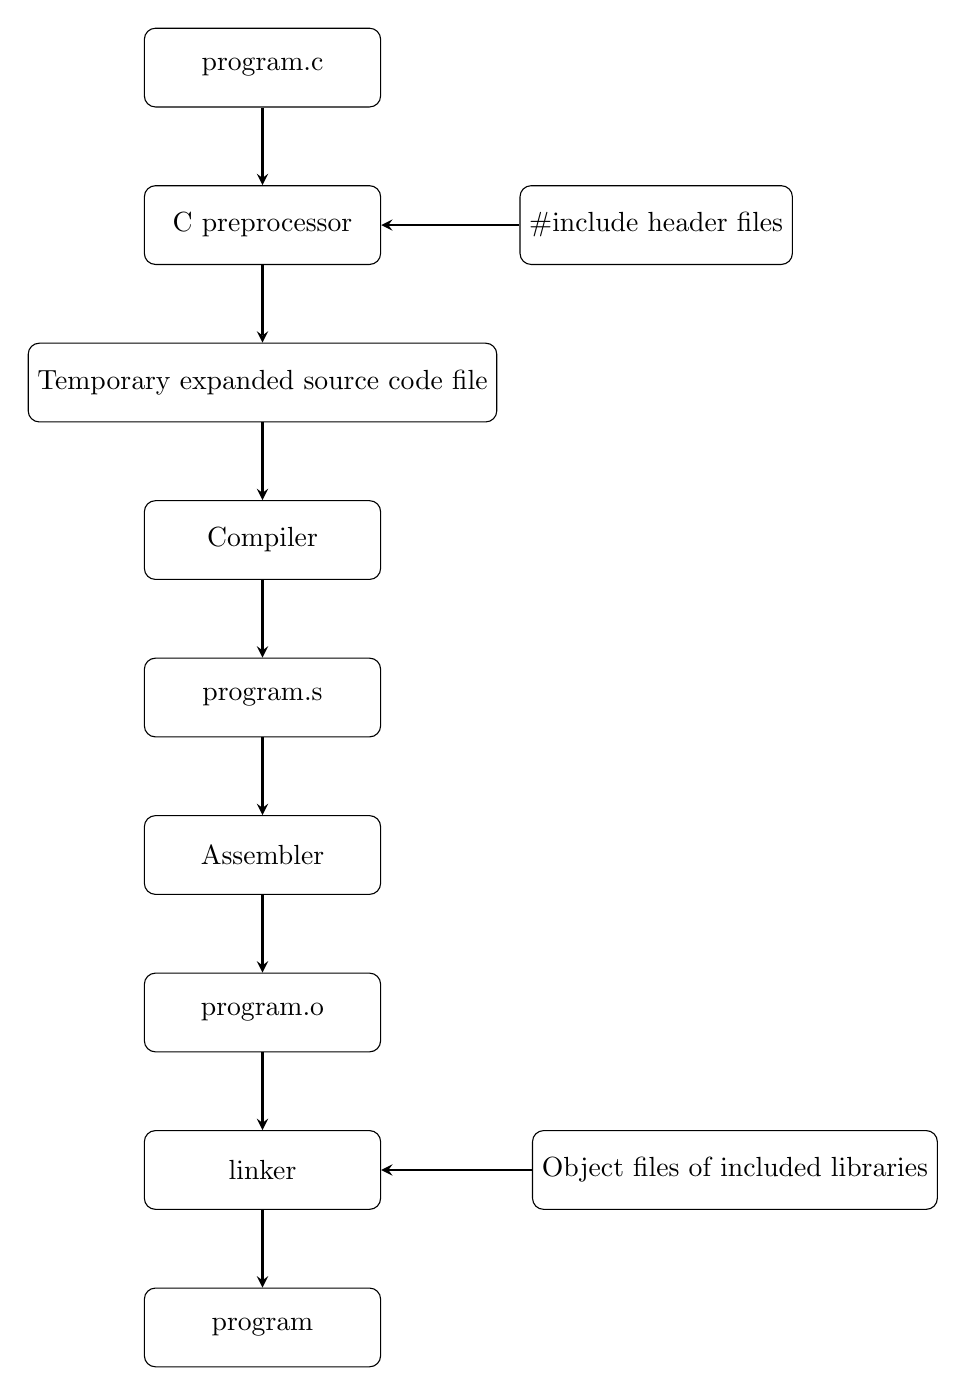
\begin{tikzpicture}[node distance=2cm]
	%defines
	\tikzstyle{programc} = [rectangle, rounded corners, minimum width=3cm, minimum height=1cm,text centered, draw=black]
	\tikzstyle{cPreProcessor} = [rectangle, rounded corners, minimum width=3cm, minimum height=1cm,text centered, draw=black]
	\tikzstyle{includeHeaderFiles} = [rectangle, rounded corners, minimum width=3cm, minimum height=1cm,text centered, draw=black]
	\tikzstyle{temporaryFile} = [rectangle, rounded corners, minimum width=3cm, minimum height=1cm,text centered, draw=black]
	\tikzstyle{compiler} = [rectangle, rounded corners, minimum width=3cm, minimum height=1cm,text centered, draw=black]
	\tikzstyle{programS} = [rectangle, rounded corners, minimum width=3cm, minimum height=1cm,text centered, draw=black]
	\tikzstyle{assembler} = [rectangle, rounded corners, minimum width=3cm, minimum height=1cm,text centered, draw=black]
	\tikzstyle{programO} = [rectangle, rounded corners, minimum width=3cm, minimum height=1cm,text centered, draw=black]
	\tikzstyle{linker} = [rectangle, rounded corners, minimum width=3cm, minimum height=1cm,text centered, draw=black]
	\tikzstyle{objectOfHeaders} = [rectangle, rounded corners, minimum width=3cm, minimum height=1cm,text centered, draw=black]
	\tikzstyle{program} = [rectangle, rounded corners, minimum width=3cm, minimum height=1cm,text centered, draw=black]
	\tikzstyle{arrow} = [thick,->,>=stealth]
	%chart
	\node (programc) [programc] {program.c};
	\node (cPreProcessor) [cPreProcessor, below of=programc] {C preprocessor};
	\node (includeHeaderFiles) [includeHeaderFiles, right of=cPreProcessor, node distance=5cm] {\#include header files};
	\node (temporaryFile) [temporaryFile, below of=cPreProcessor] {Temporary expanded source code file};
	\node (compiler) [compiler, below of=temporaryFile] {Compiler};
	\node (programS) [includeHeaderFiles, below of=compiler] {program.s};
	\node (assembler) [assembler, below of=programS] {Assembler};
	\node (programO) [programO, below of=assembler] {program.o};
	\node (linker) [linker, below of=programO] {linker};
	\node (objectOfHeaders) [objectOfHeaders, right of=linker, node distance=6cm] {Object files of included libraries};
	\node (program) [compiler, below of=linker] {program};
	\draw [arrow] (programc) -- (cPreProcessor);
	\draw [arrow] (includeHeaderFiles) -- (cPreProcessor);
	\draw [arrow] (cPreProcessor) -- (temporaryFile);
	\draw [arrow] (temporaryFile) -- (compiler);
	\draw [arrow] (compiler) -- (programS);
	\draw [arrow] (programS) -- (assembler);
	\draw [arrow] (assembler) -- (programO);
	\draw [arrow] (programO) -- (linker);
	\draw [arrow] (objectOfHeaders) -- (linker);
	\draw [arrow] (linker) -- (program);
\end{tikzpicture}
	\caption{Compilation process from High programming language to an executable file \cite{CLanguage}}\label{fig:compilationProcess}
\end{figure}
				\paragraph{C programming:}
Bell Labs developed C in the early 1970's with the UNIX OS. The book ''The C Programming Language'' \cite{CLanguage}, published in 1978, was for many years the standard reference for the C language. In 1988 a second edition of ''The C Programming Language'' was published, caused by the C language usage spreading beyond UNIX system. This second edition included a changed, platform-independent, standard. C became a general purpose programming language close to the machine hardware, using pointers to locate variables on a specific place in memory.

Header files are files with the extension ''.h'', those files contain function declarations to library source files. Every C program uses header files. Program \ref{lst:CHelloWorld} \cite{CLanguage} includes the stdio library by typing ''\#include'' followed with the library name. Library stdio provides the function printf(), used as an easy way of printing to the console. Next there is a line starting with ''int main'', called the main function. Declaration type ''int'' before main indicates the return type, main will always return an integer. When the executable exits without an error, main will return a zero, otherwise another integer defined by the occurred error. That's the reason why in program \ref{lst:CHelloWorld} a zero is returned in the end of the main function. Two function parameters ''argc'' and ''argv'' must always be provided, these are named command line arguments. Those are used to give initial values to the main function. Argument ''argc'' will be the number of characters pointed to by ''argv'', remind that the first char will always be a space separating the executable and the arguments. As already discussed, ''printf()'' will print the string ''Hello world! \textbackslash n''. Where ''\textbackslash n'' represents a new line in the console windows.
\centering
\begin{lstlisting}[caption={C Hello world! \cite{CLanguage}},label={lst:CHelloWorld},language=C, float=h]
#include <stdio.h>
int main(int argc, char ** argv) {
   printf("Hello world!\n");
   return 0;
}
\end{lstlisting}
The C language has several types of variables, some basic types are:
\begin{itemize}
	\item Integers:	which can be both positive or negative numbers (char, int, short, long or long long)
	\item Unsigned integers:	contributing only the positive integers (unsigned char, unsigned int, unsigned long or unsigned long long)
	\item Floating point numbers:	are real numbers with a, integer before and after the comma (float or double)
\end{itemize}
Variables can be declared with and without initialisation. Program \ref{lst:decIni} shows declaration without initialisation of integer ''foo'' and declaration with initialisation of double ''bar''. Programming languages variables differ with Verilog HDL wires or registers in the fact that variables do not require to be initialised when not used. While wires and registers in Verilog HDL do, like mentioned in \ref{par:Verilog} paragraph Verilog. 
\begin{lstlisting}[caption={Integer declaration and initialisation},label={lst:decIni},language=C]
int foo;
double bar = 1,5;
\end{lstlisting}
The execution of a C program is completed by one line at a time. So the next line will not be started unless the previous line was completed with success. Program \ref{lst:cExample} verifies this statement. Function ''timerStart()'' starts a timer counting the passed seconds, ''printf()'' prints immediately the value of integer a and the passed time. When executing the program the first printf can immediately be seen in the console, time is still 0 seconds and the value of ''a'' will be two. Variable ''a'' will not be zero, because it is changed to two just before the printf function can be executed. After 1 000 000 microseconds a second ''printf'' is executed, printing the variable a = 5 and passedTime = 1 second. This example program proves that the variable ''a'' can be changed a lot of times in the same program, but only line after line as they are programmed. Compared with a HDL running on an FPGA, referring to figure \ref{fig:races}, races will happen and the variable ''a'' would be changed to a lot of numbers at the same time and in an uncontrolled manner.
\begin{lstlisting}[caption={C example program to verify the ''one line executes at a time'' statement},label={lst:cExample},language=C, float=h]
#include <stdio.h>

int main(int argc, char ** argv) {
   int a = 0;
   int passedTime = 0;
   timerStart();
   a = 2;
   printf(''a = \%d when passedTime = \%d second'',a, passedTime);
   a = 3;
   usleep(1000000); // 1 second
   a = 5;
   printf(''a = \%d when passedTime = \%d second'',a, passedTime);
   timerEnd();
   return 0;
}

Output in shell:
   a = 2 when passedTime = 0 s
   a = 5 when passedTime = 1 s
\end{lstlisting}
				\paragraph{OpenCL host:} \label{par:OpenCLHost}
A general description about OpenCL can be found in subsection \ref{subsec:OpenCL}, this paragraph will handle the OpenCL host program. The OpenCL host needs to invoke ''clEnqueueTask()'' for OpenCL kernel execution, but before the host is able to run ''clEnqueueTask()'' a kernel environment must to be configured. So the organiser of the program, performing all next 13 tasks \cite{OpenCLHelloWorld} to configure, initiate, catch results and finish the OpenCl kernel.
\begin{enumerate}
	\item Get a list of available platforms:	A platform is defined as the brand of devices such as Intel or AMD. OpenCL detects which platforms are available and stores them in variable ''platform\_id''. The first parameter of clGetPlatformIDs defines how many platforms are wanted, obviously this parameter needs to be greater than zero.
\begin{lstlisting}%[caption={Get a list of available platforms},label={lst:availablePlatform},language=C]
[language=C, float=h]
   cl_platform_id platform_id = NULL;
   cl_uint ret_num_platforms;
   ret = clGetPlatformIDs(1, &platform_id, &ret_num_platforms);
\end{lstlisting}

	\item Select device:	Devices are the products of a brand, like CPU's, GPU's or FPGA's. They belong to a specific platform. If multiple devices of different platforms are used, this step needs to be combined with step one. First clGetDeviceIDs receives an id representing an available platform and next a device type needs to specified. Device types can only be one of the following: CL\_DEVICE\_TYPE\_CPU, CL\_DEVICE\_TYPE\_GPU, CL\_DEVICE\_TYPE\_ACCELERATOR, CL\_DEVICE\_TYPE\_DEFAULT or CL\_DEVICE\_TYPE\_ALL. The first three device types correspond to using the CPU, GPU and FPGA. Function parameter three specifies the number of devices the host would like to use. ''ret\_num\_devices'' returns the amount devices available of the specified device type.
\begin{lstlisting}%[caption={Select device},label={lst:selectDevice},language=C]
[language=C, float=h]
   cl_device_id device_id = NULL;
   cl_uint ret_num_devices;
   ret = clGetDeviceIDs(platform_id, CL_DEVICE_TYPE_DEFAULT,
   1, &device_id, &ret_num_devices);
\end{lstlisting}

	\item Create Context:	Objects use a context in OpenCL. Why and what the context does will be explained in memory objects. To create the context clCreateContext needs to know how many and which devices needs a context, respectively in parameters two and three. All the other parameters represent advanced properties that are not discussed in this thesis.
\begin{lstlisting}%[caption={Create Context},label={lst:createContext},language=C]
[language=C, float=h]
   cl_context context = NULL;
   context = clCreateContext(NULL, 1, &device_id,
   NULL, NULL, &ret);
\end{lstlisting}

	\item Create command queue:	When a device is active, a medium to communicate with the device must be created. OpenCL calls this medium a command queue. The command Queue needs arguments, in this order, to specify: the used context, which device will be executed in this command queue and some not discussed advanced parameters.
\begin{lstlisting}%[caption={Create command queue},label={lst:createCommandQueue},language=C]
[language=C, float=h]
   cl_command_queue command_queue = NULL;
   command_queue = clCreateCommandQueue(context,
   device_id, 0, &ret);
\end{lstlisting}

	\item Create memory objects:	Kernels can't access memory outside their device. A solution is found by copied the data from host to device memory. OpenCL uses a buffer as medium to copy the data back and forward. ''clCreateBuffer'' needs to know which context to use and the access rights the kernel has to the allocated device memory. As third argument is the occupied memory size passed.
\begin{lstlisting}%[caption={Create memory objects},label={lst:createMemoryObjects},language=C]
[language=C, float=h]
   cl_mem memobj = NULL;
   memobj = clCreateBuffer(context, CL_MEM_READ_WRITE,
   MEM_SIZE * sizeof(char), NULL, &ret);
\end{lstlisting}

	\item Read kernel file:	In this step, things need to be split up. When a CPU or GPU is used, the OpenCL kernel can be read from source file. In contrary for the FPGA, Altera desires to offline compile OpenCL kernels to a raw binary file. This and the next step mention the constructions for both Apple and Altera platforms.
		\begin{itemize}
			\item Apple: The host program reads the OpenCL kernel file and puts the file in a huge array of characters with an allocated size of MAX\_SOURCE\_SIZE. An array of character in C is comparable with a string datatype.
\begin{lstlisting}%[caption={Read kernel file},label={lst:availablePlatform},language=C]
[language=C, float=h]
   FILE *fp;
   char fileName[] = "./hello.cl";
   char *source_str;
   size_t source_size;
 
   /* Load kernel code */
   fp = fopen(fileName, "r");
   if (!fp) {
      fprintf(stderr, "Failed to load kernel.\n");
      exit(1);
   }
   source_str = (char*)malloc(MAX_SOURCE_SIZE);
   source_size = fread(source_str, 1, MAX_SOURCE_SIZE, fp);
   fclose(fp);
\end{lstlisting}
			\item Altera: Because the SoC is primitive Altera desires to offline compile the object file with a specific license. To load the binary file, parameter KERNEL\_NAME should contain the path to the binary file in the SoC directory. A last parameter defines the device where the kernel is installed.
\begin{lstlisting}%[caption={Read kernel file},label={lst:availablePlatform},language=C]
[language=C, float=h]
   std::string binary_file = getBoardBinaryFile(KERNEL_NAME,
   device);
\end{lstlisting}
		\end{itemize}
		
	\item Create program object:	A kernel program can contain multiple kernel functions. If there are multiple kernel functions, each kernel should be converted to an object by the codes below.
		\begin{itemize}
			\item Apple: Once the source code is read from the kernel source file, it must be processed into an OpenCL kernel program. Function ''clCreateProgramWithSource'' creates a program object file in variable ''program''.
\begin{lstlisting}%[caption={Create program object},label={lst:createProgramObject},language=C]
[language=C, float=h]
   cl_program program = NULL;
   program = clCreateProgramWithSource(context, 1, (const char **)&source_str, (const size_t *)&source_size, &ret);
\end{lstlisting}
			\item Altera: After the offline compilation a binary file was created. In the previous step the binary file was loaded into the host program. Now ''createProgramFromBinary'' converts the binary to an object file in variable ''program''. 
\begin{lstlisting}%[caption={Read kernel file},label={lst:availablePlatform},language=C]
[language=C, float=h]
   program = createProgramFromBinary(context,
   binary_file.c_str(), &device, 1);
\end{lstlisting}
		\end{itemize}
	
	\item Compile kernel:	At this point the kernel program needs to be build for a specific device with ''clBuildProgram''. In the step above ''clCreateProgramWithBinary'' could be used instead of the ''clCreateProgramWithSource'', that way ''clBuildProgram'' would not be necessary for the Altera program kernel.
\begin{lstlisting}%[caption={Compile kernel},label={lst:compileKernel},language=C]
[language=C, float=h]
   ret = clBuildProgram(program, 1, &device_id, NULL,NULL, NULL);
\end{lstlisting}
	
	\item Create kernel object:	For each kernel function an object should be created. The second argument of function ''clCreateKernel'' sets the name of the kernel object. In this case there is only one kernel, but when needed multiple kernel objects could be generated.
\begin{lstlisting}%[caption={Create kernel object},label={lst:createKernelObject},language=C]
[language=C, float=h]
   cl_kernel kernel = NULL;
   kernel = clCreateKernel(program, "hello", &ret);
\end{lstlisting}

	\item Set kernel arguments:	Setting kernel arguments is the main task of the OpenCL host program. The kernel expects a pointer to the memory objects, this pointer should be declared in the host side. When the pointer is not declared on the host side, the host can't manage the memory. The first argument is the kernel object itself, secondly the number of which argument will be set is specified. Next the argument size and pointer to the argument are passed.
\begin{lstlisting}%[caption={Set kernel arguments},label={lst:setKernelArguments},language=C]
[language=C, float=h]
   ret = clSetKernelArg(kernel, 0, sizeof(cl_mem),
   (void *) &memobj);
\end{lstlisting}

	\item Execute kernel:	The kernel will be executed when this function is started. Function ''clEnqueueTask'' takes the kernel and launches it into the queue. In this example we have only one, so the fifth argument can be ''NULL''. Otherwise the fifth argument must be set as an event object, the event object will wait for the kernel to finish execution to throw the host an event.
\begin{lstlisting}%[caption={Execute kernel},label={lst:executeKernel},language=C]
[language=C, float=h]
   ret = clEnqueueTask(command_queue, kernel, 0,
   NULL, NULL);
\end{lstlisting}

	\item Read memory object:	Once the kernel is finished, return data must be read from the kernel. The return data will be available on the device side, where ''clEnqueueReadBuffer'' can copy the data back to the host side. This function uses a lot of arguments, but only some of them are important. The second argument points to the device side memory, while sixth argument points to the host side memory and the fifth argument determines the memory size.
\begin{lstlisting}%[caption={Read memory object},label={lst:readMemoryObject},language=C]
[language=C, float=h]
   char string[MEM_SIZE];
   ret = clEnqueueReadBuffer(command_queue, memobj,
   CL_TRUE, 0, MEM_SIZE * sizeof(char), string, 0,NULL, NULL);
\end{lstlisting}

	\item Free objects:	Like in a regular C program, all objects needs to be freed.
\begin{lstlisting}%[caption={Free objects},label={lst:freeObjects},language=C]
[language=C, float=h]
   ret = clReleaseKernel(kernel);
   ret = clReleaseProgram(program);
   ret = clReleaseMemObject(memobj);
    ret = clReleaseCommandQueue(command_queue);
   ret = clReleaseContext(context);
\end{lstlisting}
\end{enumerate}
This was a short introduction. When OpenCL is used in a application, the kernel is repetitive executed in a contiguous cycle. A cycle about copying data from host to kernel, executing kernel and copying data back from kernel to host, as can be seen in figure \ref{fig:OpenCLApplicationCycle}. 

\begin{figure}\centering
	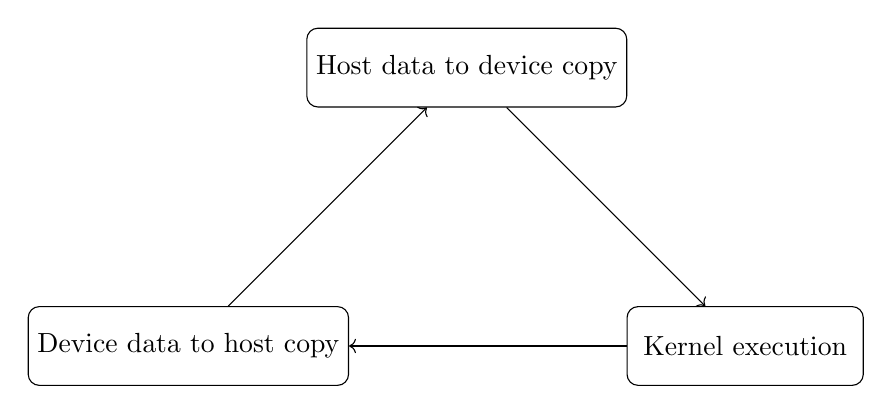
\begin{tikzpicture}[node distance=5cm]
	%defines
	\tikzstyle{hostToDevice} 	= [rectangle, rounded corners, minimum width=3cm, minimum height=1cm,text centered, draw=black]
	\tikzstyle{kernelExecution}	= [rectangle, rounded corners, minimum width=3cm, minimum height=1cm,text centered, draw=black]
	\tikzstyle{deviceToHost}	= [rectangle, rounded corners, minimum width=3cm, minimum height=1cm,text centered, draw=black]
	\tikzstyle{arrow} = [thick,->,>=stealth]
	%chart
	\node (hostToDevice) [hostToDevice] {Host data to device copy};
	\node (kernelExecution) [kernelExecution, below right of=hostToDevice] {Kernel execution};
	\node (deviceToHost) [deviceToHost, below left of=hostToDevice] {Device data to host copy};
	\draw [->] (hostToDevice) edge (kernelExecution) (kernelExecution) edge (deviceToHost) (deviceToHost) edge (hostToDevice);
\end{tikzpicture}
	\caption{OpenCL real life applications kernel cycle}\label{fig:OpenCLApplicationCycle}
\end{figure}
%%FPGA							%%%%%%%%%%%%%%%%%%%%%%%%%%%%%%%%
		\subsection{FPGA}
FPGA abbreviation of Field Programmable Gate Arrays enable designers to program logic in the field. Altera, the manufacturer of our SoC published a book named FPGA for dummies \cite{FPGAforDummies}. Everything in this subsection is referenced by this book.

			\subsubsection{Short history}
Ten years after the first commercial processor, intel 4004 \cite{intel4004}, was released, the first FPGA's where created. They where difficult to program, expensive and had a small amount of configurable logic blocks. Most designers avoided them and used processors and/or ASICs. ASICs are Application-Specific Integrated Circuit, configured for a specific purpose. When ASICs where used, the application needed parallel data processing or the IC was produced by mass production. Caused by the high initial costs of ASICs.

These days FPGA's have more logic blocks and are much cost-effective than ASICs, but the main advantage is their endless reconfigurability after manufacturing. Even most FPGA's today can be programmed during runtime \cite{FPGAruntimeProgramming}, meaning they have the ability to partly reprogram for a different use.
			\subsubsection{FPGA design flow}
Developing a FPGA implementation includes 5 main stages, figure\ref{fig:fpgaDesignFlow}. It all starts with a system design. Engineers decide which functions have to be implemented. They also keep the integration with the rest of the system in mind. Secondly all the needed inputs and outputs of the FPGA are matched to the other components in the system to inform the pin planner. The name Pin planner is self explaining, planning which pins of the inputs and outputs are connected to which components on the PCB. The next stage is the most time consuming phase. Here designers program in a HDL like Verilog, VHDL or a schematical editor to describe the logic circuit. Designers can implement IP-blocks, Intellectual Property blocks, to interact with the HDL. Some IP-blocks come with the program, others need to be bought by thirty party companies. Once the design is complete, two possibilities are left. When the design is considered small, developers start testing on the FPGA. If testing directly on FPGA is impossible or when dealing with a large design, test benches are desired. A test bench simulates the HDL as functional verification of the system. Although a HDL is tested by a test bench, there might still be errors after implementation. A test bench is as good as the test bench designer. Once the design has been defined, tested or not, synthesis is started. Synthesis start checking the code on typo's, not included packages, name mismatches, registers that needs to be wires, etc. Once checking is complete, synthesis will optimise the code. The last step, shown in figure\ref{fig:fpgaDesignFlow}, is the design verification. Design verification handles the feeding of bitstream files to the FPGA and testing the whole system implementation.
\begin{figure}\centering
	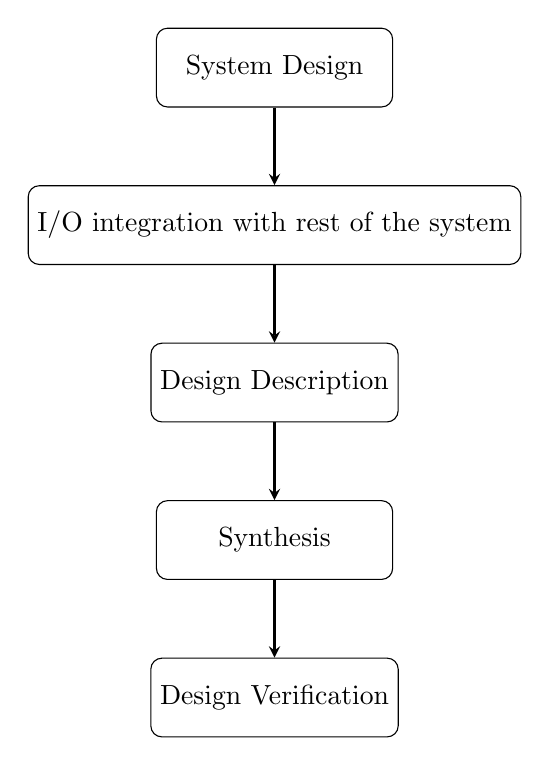
\begin{tikzpicture}[node distance=2cm]
	%defines
	\tikzstyle{systemDesign} = [rectangle, rounded corners, minimum width=3cm, minimum height=1cm,text centered, draw=black]
	\tikzstyle{ioIntegration} = [rectangle, rounded corners, minimum width=3cm, minimum height=1cm,text centered, draw=black]
	\tikzstyle{designDescription} = [rectangle, rounded corners, minimum width=3cm, minimum height=1cm,text centered, draw=black]
	\tikzstyle{synthesis} = [rectangle, rounded corners, minimum width=3cm, minimum height=1cm,text centered, draw=black]
	\tikzstyle{designVerification} = [rectangle, rounded corners, minimum width=3cm, minimum height=1cm,text centered, draw=black]
	\tikzstyle{arrow} = [thick,->,>=stealth]
	%chart
	\node (systemDesign) [systemDesign] {System Design};
	\node (ioIntegration) [ioIntegration, below of=systemDesign] {I/O integration with rest of the system};
	\node (designDescription) [designDescription, below of=ioIntegration] {Design Description};
	\node (synthesis) [synthesis, below of=designDescription] {Synthesis};
	\node (designVerification) [designVerification, below of=synthesis] {Design Verification};
	\draw [arrow] (systemDesign) -- (ioIntegration);
	\draw [arrow] (ioIntegration) -- (designDescription);
	\draw [arrow] (designDescription) -- (synthesis);
	\draw [arrow] (synthesis) -- (designVerification);
\end{tikzpicture}
	\caption{FPGA design flow}\label{fig:fpgaDesignFlow}
\end{figure}
%%Hardware Description Languages	%%%%%%%%%%%%%%%%%%%%%%%%%%%%%%%%
			\subsubsection{Hardware Description Languages}
				\paragraph{Verilog:} \label{par:Verilog}
As mentioned earlier, HDLs describe digital hardware. Which means there is hardware configured inside the IC and we need to handle the source code like it is hardware. There are two main HDL languages: Verilog and VHDL. Since we only used Verilog in our thesis, VHDL will not be discussed.

Every programming language uses variables. Verilog uses two main kind of variables, wires ''wire'' and registers ''reg''. A ''wire'' is directly a wire in the IC and is used in assignments or modules. Which means that assignments and modules have strong connections between each other. While registers are considered weak connections. ''regs'' are only used when a signal changes inside an always statement. But unlike regular programming languages, a signal named clock is used. The clock signal is the most important signal in Verilog. When horses A, B and C racing against each other on different racetracks, they will probably never finish at the same time. Imagine the horses being electric pulses A, B and C. There will happen races between the three pulses and for the each stage, but all pulses need to be read at the same time. That's where the clock signal comes in. On the positive edge of the clock, referring to figure\ref{fig:races}, all signals leave register1 at the positive edge of the clock. Obviously signal A will be the first to reach register2 and there will start a race between pulse A, B and C to get the second and third place of B and C in register2. Who will arrive first is unpredictable, because of the different delays in and between between the random placed logic elements. Using a clock makes sure there will be enough time for every signal to arrive.

Besides the clock, the system needs a default state. When the reset signal is engaged, the whole system is set to default. A reset can happen synchronously (Program \ref{lst:VerilogSynReset}) or asynchronously (Program \ref{lst:VerilogAssynReset}), meaning respectively resetting only at the edge of the clock or resetting whenever the reset signal is engaged. The only difference between the two is the added ''posedge reset'' in Program \ref{lst:VerilogSynReset}. When a designer is not consequent and changes between synchronous and asynchronous reset or places another signal in the always construct, the behaviour will probably be unpredictable.

Inside ''always'' if, case, while, for and repeat statements can be used. All used signals inside an always need to be declared as registers ''reg'' and need to have a default value defined in ''if(reset)''.

Outside ''always'' two possibilities can be considered. The first one is an assignment between wires and the second one is wiring another module into the current module. Assignments are used when a signal needs to be delivered immediately when it is present two examples can be seen in Program \ref{lst:VerilogAssignment}. Assignment to ''result1'' is a logical or between two wires ''a'' and ''b''. While ''result2'' looks like an if-else statement without clock. Whenever ''conditionBit'' is true, the ''valueBit'' will be returned in wire ''return2'', otherwise ''valueFalse'' will be returned. Designers need to remind that in an assignment no clock is used. So when not carefully handled races occur which results in unpredictable behaviour. Another possibility to using assignments is to connect a register and a wire together. Secondly a module can be used inside another module like in Program \ref{lst:VerilogModule}, where object ''objectAbc'' of module ''abc'' is wired to wires ''A'', ''B'' and ''C''. The inputs and outputs of module abc are ''a'', ''b'' and ''c''.

Verilog-syntax is very simple, we discussed already almost all the important syntax except how modules look like. A module is based on regs, wires, assignments, alwayses, other modules, inputs, outputs and inouts. The last three have some special rules. An input must always be of type net, when used external they may be connected to regs or wires. Outputs have the opposite rules. Inside the module they can be a wire or reg, but externally the outputs must be connected to a wire. Lastly inouts are always wires internally and externally. An elementary example of a module can be found in Program \ref{lst:elementaryVerilogModule}.
\begin{figure}
	\centering
	\begin{circuitikz}
	%register1
	\draw (-4,0) -- (-4,4) -- (-3,4) -- (-3,0) -- cycle;
	\draw (-4,1) -- (-3,1);
	\draw (-4,2) -- (-3,2);
	\draw (-4,3) -- (-3,3);
	\node at (-3.5,3.5) {$clock$};
	\node at (-3.5,2.5) {$A$};
	\node at (-3.5,1.5) {$B$};
	\node at (-3.5,0.5) {$C$};
	\node at (-3.5,-0.5) {$register1$};
	%and gate
	\node[european and port] at (-1,1.225) (andGate) {};
	%or gate
	\node[european or port] at (1,1.5) (orGate) {};
	%connections
	\draw (-0.77,2.5) -- (orGate.in 1);
	\draw (andGate.out) -- (orGate.in 2);
	\draw (-3,1.5) -- (andGate.in 1);
	\draw (-3,0.5) -- (-2.77,0.5);
	\draw (-2.77,0.5) -- (andGate.in 2);
	\draw (-3,2.5) -- (3,2.5);
	\draw (orGate.out) -- (3,1.5);
	\draw (andGate.out) -- (-0.8,0.5);
	\draw (-0.8,0.5) -- (3,0.5);
	%register2
	\draw (4,0) -- (4,4) -- (3,4) -- (3,0) -- cycle;
	\draw (4,1) -- (3,1);
	\draw (4,2) -- (3,2);
	\draw (4,3) -- (3,3);
	\node at (3.5,3.5) {$clock$};
	\node at (3.5,2.5) {$A$};
	\node at (3.5,1.5) {$B$};
	\node at (3.5,0.5) {$C$};
	\node at (3.5,-0.5) {$register2$};
\end{circuitikz}
	\caption{HDL races figure}
	\label{fig:races}
\end{figure}
\begin{lstlisting}[caption={Verilog example, synchronous reset},label={lst:VerilogSynReset},language=Verilog, float=h]
   always @(posedge clk) begin
      if(reset)
         ... <= 1'b0;
      else
         ... <= ...;
    end
\end{lstlisting}
\begin{lstlisting}[caption={Verilog example, assynchronous reset},label={lst:VerilogAssynReset},language=Verilog, float=h]
   always @(posedge clk or posed reset) begin
      if(reset)
         ... <= 1'b0;
      else
         ... <= ...;
   end
\end{lstlisting}
\begin{lstlisting}[caption={Verilog example assignments},label={lst:VerilogAssignment},language=Verilog, float=h]
	assignment result1 = a or b;
	assignment result2 = (conditionBit) ? valueTrue : valueFalse;
\end{lstlisting}
\begin{lstlisting}[caption={Verilog example, using a module},label={lst:VerilogModule},language=Verilog, float=h]
   abc objectAbc (
      .a(A);
      .b(B);
      .c(C)
   );
\end{lstlisting}
\begin{lstlisting}[caption={Verilog example, defining a module},label={lst:elementaryVerilogModule},language=Verilog, float=h]
   module abc ( a, b, c );
      input	a;
      input	b;
      output	c;
	
      assign c = a and b;
   endmodule
\end{lstlisting}
				\paragraph{OpenCL kernel:}\label{par:OpenCLKernel}
An OpenCL kernel is a C/C++ based programming language to rapidly extend a compute exhausting task to a hardware accelerator, such as a GPU or in our case a FPGA. In order to use a kernel, a host in C or C++ should be coded. The host side, explained in \ref{par:OpenCLHost} paragraph OpenCL Host, checks and configures the environment before initiating the kernel. Kernels are initiated on a device of a specific platform. In our case, the device is an FPGA. FPGA's are ideal devices for algorithms that parallelise their problems. We will explain how the kernel works based on figure \ref{fig:kernelSchoolLayout} as a representative example of a school calculating a sum or multiplications. The representative example will be linked with the real kernel using figure \ref{fig:kernelLayout}. Imagine a very large sum of multiplications, like equation \ref{eq:kernelSchool}, calculated by a school.
\begin{equation} \label{eq:kernelSchool}
   result=(A*B+C*D+E*F+G*H)+(I*J+K*L+M*N+O*P)
\end{equation}
There could be one person doing all the multiplications and adding them to the previous ones, but he will be take a long time doing the same thing over and over again. It would be easier if the school extends parts of the calculation to different departments, as can be seen in figure \ref{fig:kernelSchoolLayout}. Department A takes the first 8 numbers and department B the last 8 numbers. Each department distributes the multiplications to classes of two students. A student goes to the board in front of the class, calculates the multiplication and returns the result to the board. Once all the students are finished, the teacher of the class return the results to the department. Where the department waits for all the other classes to finish and calculates the sum of all results. When each department returned their sums, the school director can calculate the sum of all values returned by the departments.

Figure \ref{fig:kernelLayout} represents the real kernel situation of the previous example. The outer circle represents the vendors platform, like Intel/AMD/Altera. Vendors platform could be seen as the campus, with different schools doing a specific parallelised algorithm, called a kernel. Devices belong to a vendors platform, but that is not important. It is just a practical way of structuring devices and managing device driverscode for all vendors. Each device has it's own global memory which is the only memory the host side has access to, so all input and output data are passed here. Besides the memory needed by the device at least one department, equal to a compute unit, is mandatory to calculate the calculation. Our school example uses two departments A and B. Compute units are able to work directly with global memory data, but they are more efficient when data is passed to local memory. The difference between local and global memory is the speed and their size. Global memory is bigger than local memory, but local memory is faster than global memory. So the department should always copy their data from global to local memory. Local memory can be represented as the commune board in front of the class. Every student can take a note from the board, calculate and return his result to the board. Notes are taken into private memory and after a work item, student, is finished calculating returned to local memory. When all workgroups are finished a ''master workgroup'' is assigned to do the job of the school director, calculating a final sum over all the departments returned results.
\begin{figure}\centering
	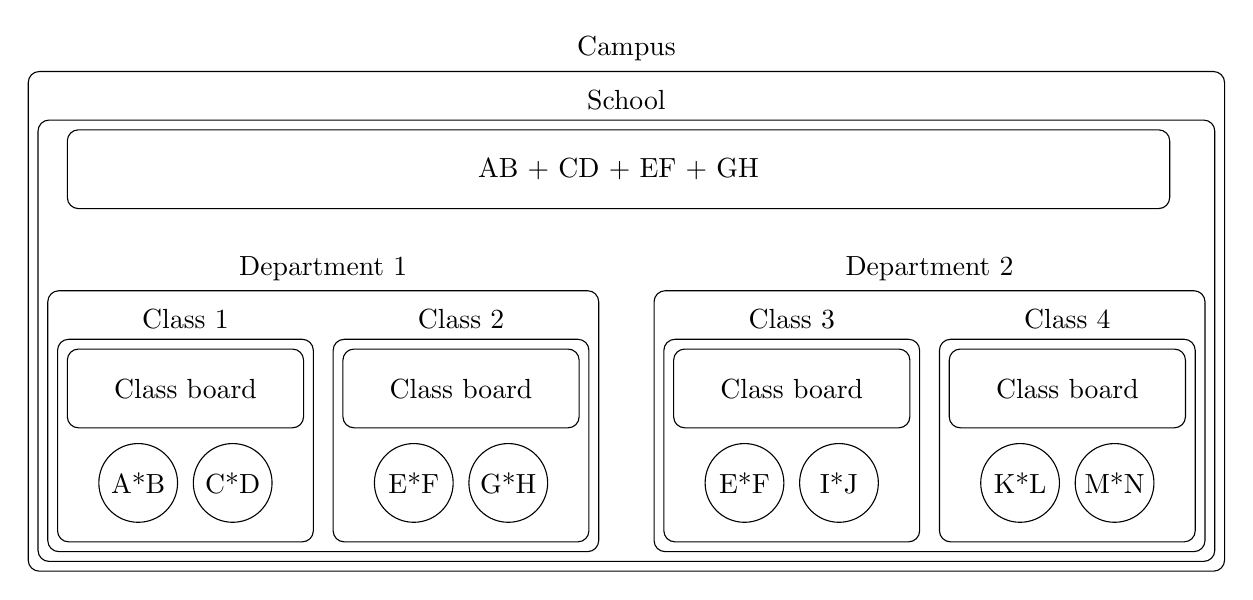
\begin{tikzpicture}[
  node distance=7mm,
  title/.style={font=\fontsize{6}{6}\color{black!50}\ttfamily},
  typetag/.style={rectangle, draw=black!50, font=\scriptsize\ttfamily, anchor=west}
]
	\tikzstyle{workgroup1} = [rectangle, rounded corners, minimum width=3cm, minimum height=1cm,text centered, draw=black]
	\tikzstyle{workgroup2} = [rectangle, rounded corners, minimum width=3cm, minimum height=1cm,text centered, draw=black]
	\tikzstyle{localMemory1} = [rectangle, rounded corners, minimum width=3cm, minimum height=1cm,text centered, draw=black]
	\tikzstyle{localMemory2} = [rectangle, rounded corners, minimum width=3cm, minimum height=1cm,text centered, draw=black]
	\tikzstyle{computeUnit1} = [rectangle, rounded corners, minimum width=3cm, minimum height=1cm,text centered, draw=black]

	\node[matrix] (workItem1A) {
		\draw (0.3,0.3) circle (0.5) node {A*B}; \\
	};
	\node[matrix,right of=workItem1A, node distance=12mm] (workItem1B) {
		\draw (0.3,0.3) circle (0.5) node {C*D}; \\
	};
	\node (localMemory1) [localMemory1, above of=workItem1A, node distance=12mm, xshift=6mm] {Class board};
	\node (workgroup1) [workgroup1, label={[name=workgroup1label] Class 1}, anchor=south, fit={(workItem1A) (workItem1B) (localMemory1)}] {};
	
	\node[matrix, right of=workItem1A, node distance=35mm] (workItem2A) {
		\draw (0.3,0.3) circle (0.5) node {E*F}; \\
	};
	\node[matrix,right of=workItem2A, node distance=12mm] (workItem2B) {
		\draw (0.3,0.3) circle (0.5) node {G*H}; \\
	};
	\node (localMemory2) [localMemory2, above of=workItem2A, node distance=12mm, xshift=6mm] {Class board};
	\node (workgroup2) [workgroup2, label={[name=workgroup2label] Class 2}, anchor=south, fit={(workItem2A) (workItem2B) (localMemory2)}] {};

	\node (computeUnit1) [computeUnit1, label={[name=computeUnit1label] Department 1}, anchor=south, fit={(workgroup1) (workgroup1label) (workgroup2) (workgroup2label)}] {};
	
	\tikzstyle{workgroup3} = [rectangle, rounded corners, minimum width=3cm, minimum height=1cm,text centered, draw=black]
	\tikzstyle{workgroup4} = [rectangle, rounded corners, minimum width=3cm, minimum height=1cm,text centered, draw=black]
	\tikzstyle{localMemory3} = [rectangle, rounded corners, minimum width=3cm, minimum height=1cm,text centered, draw=black]
	\tikzstyle{localMemory4} = [rectangle, rounded corners, minimum width=3cm, minimum height=1cm,text centered, draw=black]
	\tikzstyle{computeUnit2} = [rectangle, rounded corners, minimum width=3cm, minimum height=1cm,text centered, draw=black]
	
	\node[matrix, right of=workItem2B, node distance=30mm] (workItem3A) {
		\draw (0.3,0.3) circle (0.5) node {E*F}; \\
	};
	\node[matrix, right of=workItem3A, node distance=12mm] (workItem3B) {
		\draw (0.3,0.3) circle (0.5) node {I*J}; \\
	};

	\node (localMemory3) [localMemory3, above of=workItem3A, node distance=12mm, xshift=6mm] {Class board};
	\node (workgroup3) [workgroup3, label={[name=workgroup3label] Class 3}, anchor=south, fit={(workItem3A) (workItem3B) (localMemory3)}] {};
	
	\node[matrix, right of=workItem3B, node distance=23mm] (workItem4A) {
		\draw (0.3,0.3) circle (0.5) node {K*L}; \\
	};
	\node[matrix, right of=workItem4A, node distance=12mm] (workItem4B) {
		\draw (0.3,0.3) circle (0.5) node {M*N}; \\
	};
	\node (localMemory4) [localMemory4, above of=workItem4A, node distance=12mm, xshift=6mm] {Class board};
	\node (workgroup4) [workgroup4, label={[name=workgroup4label] Class 4}, anchor=south, fit={(workItem4A) (workItem4B) (localMemory4)}] {};

	\node (computeUnit2) [computeUnit2, label={[name=computeUnit2label] Department 2}, anchor=south, fit={(workgroup3) (workgroup3label) (workgroup4) (workgroup4label)}] {};
	
	
	\tikzstyle{globalMemory} = [rectangle, rounded corners, minimum width=14cm, minimum height=1cm,text centered, draw=black]
	\tikzstyle{device} = [rectangle, rounded corners, minimum width=10cm, minimum height=1cm,text centered, draw=black]
	\tikzstyle{platform} = [rectangle, rounded corners, minimum width=10cm, minimum height=1cm,text centered, draw=black]
	
	\node (globalMemory) [globalMemory, above of=computeUnit1, node distance=32mm, xshift=3.75cm] {AB + CD + EF + GH};
	\node (device) [device, label={[name=deviceLabel] School}, anchor=south, fit={(globalMemory) (computeUnit1) (computeUnit1label) (computeUnit2) (computeUnit2label)}] {};
	\node (platform) [platform, label={Campus}, anchor=south, fit={(device) (deviceLabel)}] {};
		
\end{tikzpicture}
	\caption{OpenCL kernel representative school layout}\label{fig:kernelSchoolLayout}
\end{figure}
\begin{figure}\centering
	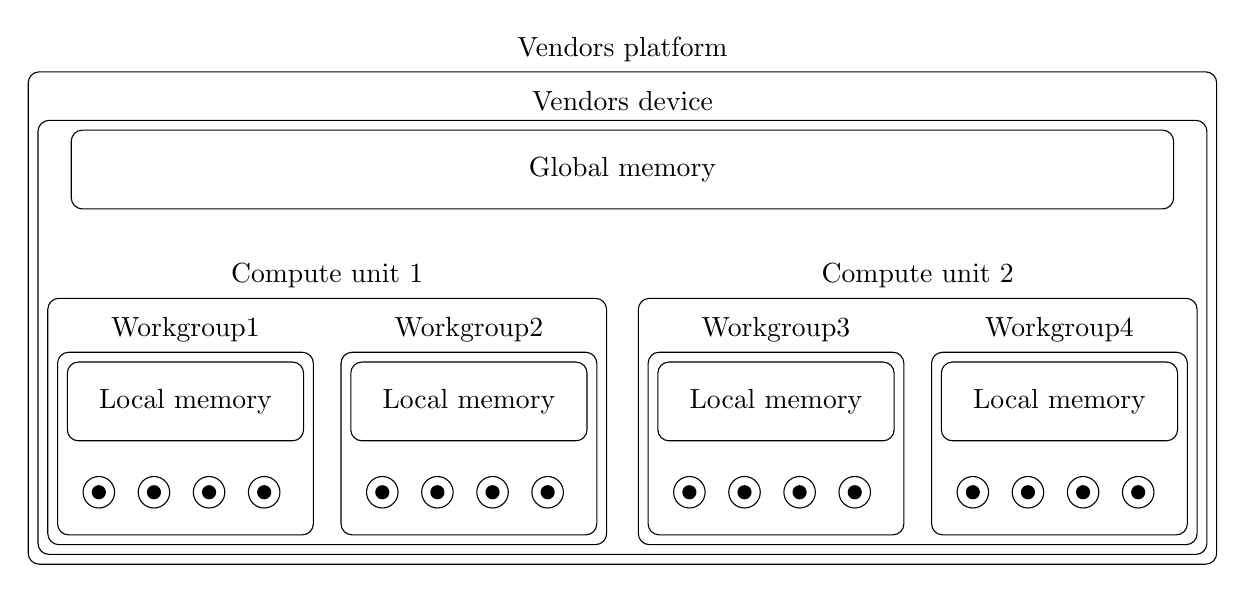
\begin{tikzpicture}[
  node distance=7mm,
  title/.style={font=\fontsize{6}{6}\color{black!50}\ttfamily},
  typetag/.style={rectangle, draw=black!50, font=\scriptsize\ttfamily, anchor=west}
]
	\tikzstyle{workgroup1} = [rectangle, rounded corners, minimum width=3cm, minimum height=1cm,text centered, draw=black]
	\tikzstyle{workgroup2} = [rectangle, rounded corners, minimum width=3cm, minimum height=1cm,text centered, draw=black]
	\tikzstyle{localMemory1} = [rectangle, rounded corners, minimum width=3cm, minimum height=1cm,text centered, draw=black]
	\tikzstyle{localMemory2} = [rectangle, rounded corners, minimum width=3cm, minimum height=1cm,text centered, draw=black]
	\tikzstyle{computeUnit1} = [rectangle, rounded corners, minimum width=3cm, minimum height=1cm,text centered, draw=black]

%	\node[matrix] (A) {
%		\draw (0,0) rectangle (1,1); 
%		\node at (0.5,0.5) {A}; \\
%	};	


	\node[matrix] (workItem1A) {
		\draw (0.3,0.3) circle (0.2);
		\fill (0.3,0.3) circle (0.09); \\
	};
	\node[matrix,right of=workItem1A, node distance=7mm] (workItem1B) {
		\draw (0.3,0.3) circle (0.2);
		\fill (0.3,0.3) circle (0.09); \\
	};
	\node[matrix,right of=workItem1B, node distance=7mm] (workItem1C) {
		\draw (0.3,0.3) circle (0.2);
		\fill (0.3,0.3) circle (0.09); \\
	};
	\node[matrix,right of=workItem1C, node distance=7mm] (workItem1D) {
		\draw (0.3,0.3) circle (0.2);
		\fill (0.3,0.3) circle (0.09); \\
	};
	\node (localMemory1) [localMemory1, above of=workItem1C, node distance=12mm, xshift=-3mm] {Local memory};
	\node (workgroup1) [workgroup1, label={[name=workgroup1label] Workgroup1}, anchor=south, fit={(workItem1A) (workItem1B) (workItem1C) (workItem1D) (localMemory1)}] {};
	
	\node[matrix, right of=workItem1D, node distance=1.5cm] (workItem2A) {
		\draw (0.3,0.3) circle (0.2);
		\fill (0.3,0.3) circle (0.09); \\
	};
	\node[matrix,right of=workItem2A, node distance=7mm] (workItem2B) {
		\draw (0.3,0.3) circle (0.2);
		\fill (0.3,0.3) circle (0.09); \\
	};
	\node[matrix,right of=workItem2B, node distance=7mm] (workItem2C) {
		\draw (0.3,0.3) circle (0.2);
		\fill (0.3,0.3) circle (0.09); \\
	};
	\node[matrix,right of=workItem2C, node distance=7mm] (workItem2D) {
		\draw (0.3,0.3) circle (0.2);
		\fill (0.3,0.3) circle (0.09); \\
	};
	\node (localMemory2) [localMemory2, above of=workItem2C, node distance=12mm, xshift=-3mm] {Local memory};
	\node (workgroup2) [workgroup2, label={[name=workgroup2label] Workgroup2}, anchor=south, fit={(workItem2A) (workItem2B) (workItem2C) (workItem2D) (localMemory2)}] {};

	\node (computeUnit1) [computeUnit1, label={[name=computeUnit1label] Compute unit 1}, anchor=south, fit={(workgroup1) (workgroup1label) (workgroup2) (workgroup2label)}] {};
	
	\tikzstyle{workgroup3} = [rectangle, rounded corners, minimum width=3cm, minimum height=1cm,text centered, draw=black]
	\tikzstyle{workgroup4} = [rectangle, rounded corners, minimum width=3cm, minimum height=1cm,text centered, draw=black]
	\tikzstyle{localMemory3} = [rectangle, rounded corners, minimum width=3cm, minimum height=1cm,text centered, draw=black]
	\tikzstyle{localMemory4} = [rectangle, rounded corners, minimum width=3cm, minimum height=1cm,text centered, draw=black]
	\tikzstyle{computeUnit2} = [rectangle, rounded corners, minimum width=3cm, minimum height=1cm,text centered, draw=black]
	
	\node[matrix, right of=workItem2D, node distance=1.8cm] (workItem3A) {
		\draw (0.3,0.3) circle (0.2);
		\fill (0.3,0.3) circle (0.09); \\
	};
	\node[matrix, right of=workItem3A, node distance=7mm] (workItem3B) {
		\draw (0.3,0.3) circle (0.2);
		\fill (0.3,0.3) circle (0.09); \\
	};
	\node[matrix, right of=workItem3B, node distance=7mm] (workItem3C) {
		\draw (0.3,0.3) circle (0.2);
		\fill (0.3,0.3) circle (0.09); \\
	};
	\node[matrix, right of=workItem3C, node distance=7mm] (workItem3D) {
		\draw (0.3,0.3) circle (0.2);
		\fill (0.3,0.3) circle (0.09); \\
	};
	\node (localMemory3) [localMemory3, above of=workItem3C, node distance=12mm, xshift=-3mm] {Local memory};
	\node (workgroup3) [workgroup3, label={[name=workgroup3label] Workgroup3}, anchor=south, fit={(workItem3A) (workItem3B) (workItem3C) (workItem3D) (localMemory3)}] {};
	
	\node[matrix, right of=workItem3D, node distance=1.5cm] (workItem4A) {
		\draw (0.3,0.3) circle (0.2);
		\fill (0.3,0.3) circle (0.09); \\
	};
	\node[matrix,right of=workItem4A, node distance=7mm] (workItem4B) {
		\draw (0.3,0.3) circle (0.2);
		\fill (0.3,0.3) circle (0.09); \\
	};
	\node[matrix, right of=workItem4B, node distance=7mm] (workItem4C) {
		\draw (0.3,0.3) circle (0.2);
		\fill (0.3,0.3) circle (0.09); \\
	};
	\node[matrix, right of=workItem4C, node distance=7mm] (workItem4D) {
		\draw (0.3,0.3) circle (0.2);
		\fill (0.3,0.3) circle (0.09); \\
	};
	\node (localMemory4) [localMemory4, above of=workItem4C, node distance=12mm, xshift=-3mm] {Local memory};
	\node (workgroup4) [workgroup4, label={[name=workgroup4label] Workgroup4}, anchor=south, fit={(workItem4A) (workItem4B) (workItem4C) (workItem4D) (localMemory4)}] {};

	\node (computeUnit2) [computeUnit2, label={[name=computeUnit2label] Compute unit 2}, anchor=south, fit={(workgroup3) (workgroup3label) (workgroup4) (workgroup4label)}] {};
	
	
	\tikzstyle{globalMemory} = [rectangle, rounded corners, minimum width=14cm, minimum height=1cm,text centered, draw=black]
	\tikzstyle{device} = [rectangle, rounded corners, minimum width=10cm, minimum height=1cm,text centered, draw=black]
	\tikzstyle{platform} = [rectangle, rounded corners, minimum width=10cm, minimum height=1cm,text centered, draw=black]
	
	\node (globalMemory) [globalMemory, above of=computeUnit1, node distance=32mm, xshift=3.75cm] {Global memory};
	\node (device) [device, label={[name=deviceLabel] Vendors device}, anchor=south, fit={(globalMemory) (computeUnit1) (computeUnit1label) (computeUnit2) (computeUnit2label)}] {};
	\node (platform) [platform, label={Vendors platform}, anchor=south, fit={(device) (deviceLabel)}] {};
		
\end{tikzpicture}
	\caption{OpenCL kernel layout: The circles represent work items with a dot in the middle as private memory}\label{fig:kernelLayout}
\end{figure}
Understanding a kernels code is more difficult than the theory described above. That's why I will only explain the kernel code, program \ref{lst:OpenCLKernelHelloWorld}, for a simple matrix addition. Three function arguments are provided, the first two are the input matrices and the third corresponds to the output matrix. To calculate the addition, each element of matrix A should be added to the corresponding element of matrix B. The sum is saved in the corresponding element of matrix R. As can be seen by ''\_\_global'', only global memory is used to store the matrices in one dimensional float arrays. In this implementation every sum is made in one workgroup with one work item. Increasing the work items per group could make the kernel execution faster in terms of parallel computation. Sometimes it takes more time to copy data from global to local memory than the execution itself. Efficient kernel design has the need for research and testing. TUT PhD student Wang Kui has written a paper about using OpenCL to rapidly prototype FPGA designs \cite{usingOpenCLToRapidalyPrototypeFPGADesigns}. He adjusted the number of work items in a workgroup and reduced hardware resource usage to replicate more OpenCL compute units.

Continuing on matrix addition example. Because kernels are another way of parallelising computation, arrays are commonly used. In order to access each element in C or C++ a for loop would be used. In OpenCL we use something equal, the function ''get\_global\_id(0)''. This function returns the number of the current workgroup, specifying which elements of the matrices should be accessed. A kernels code must be seen as the code for one element of a parallelisation.
\begin{lstlisting}[caption={OpenCL kernel example: matrix addition},label={lst:OpenCLKernelHelloWorld},language=C, float=h]
__kernel void matadd(	__global float* matrixA,
 			__global float* matrixB,
  			__global float* matrixR) {
   int i = get_global_id(0);
   matrixR[i] = matrixA[i] + matrixB[i];
}
\end{lstlisting}
%%Bridges						%%%%%%%%%%%%%%%%%%%%%%%%%%%%%%%%
		\subsection{Bridges}
Between the HPS and the FPGA three bridges, mentioned in \ref{subsec:HPS}, are used to exchange data during runtime. By default only the FPGA configuration bridge is enabled, the HPS2FPGA and FPGA2HPS bridges should be configured in Qsys. Exchanging data from HPS to FPGA and back use almost the same source code, although it was hard to find info about the FPGA2HPS bridge. Both bridges can configured with three different bus widths: 32, 64 and 128 bit.

Altera used the ARM AMBA AXI bus to implement the bridges. Both first two bridges use the ''mmap'' function, program \ref{lst:bridgesMmap}, in HPS to call a page of memory into the process's memory space \cite{HPS2FPGAManual}. Where ''memoryBaseAddress'' is the most important argument, it specifies where the bridge starts on the AXI bus. To base address is specified in Qsys, we use 0xC0000000. The base address needs to be add with an offset, for both HPS2FPGA and FPGA2HPS bridges. Explanation about the base memory offset is given in ref{subsubsec:designStructure} paragraph Qsys. The second important argument specifies the size that needs to be reserved starting from the memory base address, called ''PAGE\_SIZE''. The other parameters change with different setups. Parameter ''bridge\_map'' is the virtual mapped memory address of the bridge.
\begin{lstlisting}[caption={mmap function},label={lst:bridgesMmap},language=C, float=h]
bridge_map = mmap(NULL, PAGE_SIZE, PROT_WRITE,
   MAP_SHARED, fd, memoryBaseAddress);
\end{lstlisting}
Writing the bridges assumes basic knowledge of pointers, this can be found in \ref{subsubsec:programLanguage} paragraph C programming. The pointer valueAdress represents the location to find transmitted values. It needs an offset, specified during configuration in Qsys, to separate the AMBA AXI bus in different bridges. To write a value to the bridge, it needs to be written on the address of pointer valueAdress. Programs \ref{lst:bridgesHPS2FPGA} and \ref{lst:bridgesFPGA2HPS} show respectively the code to write the HPS2FPGA and read the FPGA2HPS bridges.
\begin{lstlisting}[caption={HPS2FPGA, transmit over bridge},label={lst:bridgesHPS2FPGA},language=C, float=h]
valueAdress = (unsigned char *) (bridgeMap + offsetHPS2FPGA);
*valueAdress = writeValue;
\end{lstlisting}
Reading is done in the same way, by transferring the pointed value of memory address ''valueAdress'' into the program.
\begin{lstlisting}[caption={FPGA2HPS, receive over bridge},label={lst:bridgesFPGA2HPS},language=C, float=h]
valueAdress = (unsigned char *) (bridgeMap + offsetFPGA2HPS);
readValue = *valueAdress;
\end{lstlisting}
			\paragraph{FPGA Configuration:	}
The FPGA can be configured in two ways. The most common way to configure the FPGA during development is to use ''Quartus programmer'', this tool uploads the SOF, SRAM Object File, to the FPGA. When a FPGA is implemented in an application, it is impossible to use Quartus programmer each time the FPGA is started. Cyclone V HPS can configure the FPGA by using the FPGA configuration bridge. Before the FPGA can be configured, all the AMBA AXI bridges must be disabled. When they are not disabled a system crash of Linux will occur. Bash program \ref{lst:setBridges0} disables the bridges. By using ''echo'' in bash, text can be written into a file. In this case is the text a ''0'' and is the file specified with a file path. Note the not yet discussed ''lwhps2fpga'', abbreviation for licht weight HPS to FPGA bridge. This one is slower than the HPS2FPGA bridge and has a fixed width of 32bit.
\begin{lstlisting}[caption={Disable the AMBA AXI bridges from HPS},label={lst:setBridges0},language=bash, float=h]
   echo 0 > /sys/class/fpga-bridge/hps2fpga/enable
   echo 0 > /sys/class/fpga-bridge/fpga2hps/enable
   echo 0 > /sys/class/fpga-bridge/lwhps2fpga/enable
\end{lstlisting}
Programming the FPGA is done by copying the Raw Binary File with ''dd'' into the device called ''fpga0''. In program \ref{lst:configureFPGADD} the dd command is shown. ''dd'' uses two arguments: ''if'' and ''of'', respectively input file and output file.
\begin{lstlisting}[caption={Configuration of the FPGA with Linux dd command},label={lst:configureFPGADD},language=bash, float=h]
   dd if=/home/root/FPGAConfigurationFile.rbf of=/dev/fpga0
\end{lstlisting}
Once the FPGA is configured, the bridges need to be enabled again. Otherwise they can't be used.
\begin{lstlisting}[caption={Enable the AMBA AXI bridges from HPS},label={lst:setBridges1},language=bash, float=h]
   echo 1 > /sys/class/fpga-bridge/hps2fpga/enable
   echo 1 > /sys/class/fpga-bridge/fpga2hps/enable
   echo 1 > /sys/class/fpga-bridge/lwhps2fpga/enable
\end{lstlisting}
%%Quartus						%%%%%%%%%%%%%%%%%%%%%%%%%%%%%%%%
		\subsection{Quartus}
			\subsubsection{Design structure}\label{subsubsec:designStructure}
				\paragraph{Pin Planner:	}
Every design needs to be fitted into the devices architecture, so do the connection to the peripherals of the embedded system. The pin planner assigns a signal name and direction to all used pins in the package. Directions can be Input, Output or Bidirectional. Table \ref{tab:pinPlanner} shows a few node names, directions and locations of the pins. Pin planner adds other information automatically during ''Assignment \& Synthesis''.
%include table 
				\paragraph{Qsys:	}
Verilog is an old and slow programming language, it is a confusing task to implement a lot of modules in the system. Qsys simplifies this in figure\ref{fig:QsysConnections}. All the included IP is shown by name and all possible connections are shown in the left column, highlighted connections are connected. Columns ''Base'' and ''End'' define the base and end address of the AMBA AXI bus used by the bridges between HPS and FPGA. Qsys generates one top module to include the whole Qsys system at once in the developer his Verilog module. All the inputs and outputs of that Qsys top module are defined in column ''export''.
\begin{figure}
	\centering
	\includegraphics[scale=0.6]{images/QsysInternalConnections.png}
	\caption{Qsys internal connections}
	\label{fig:QsysConnections}
\end{figure}
Bridges are incredible easy to configure in Qsys. There are only the choices between 32, 64 or 128 bit, figure\ref{fig:QsysBridgeConfig}. Once selected Qsys will generates all the connections. When a Qsys design includes the AMBA AXI bridges, some connections need to be added to the pin planner, luckily Quartus generates a .tcl file to add those connection to the pin assignments. But the .tcl file is only generated during the ''Assignment \& Synthesis'', so every time a AMBA AXI bridge is added, removed or changed in Qsys. Compilation process ''Assignment \& Synthesis'' followed by the .tcl file needs to be runt.
\begin{figure}
	\centering
	\includegraphics[scale=0.6]{images/QsysBridgeConfiguration.png}
	\caption{Qsys configuration of bridges}
	\label{fig:QsysBridgeConfig}
\end{figure}
				\paragraph{Compilation flow:	}
Quartus compilation flow consist of 4 steps shown in figure\ref{fig:fpgaCompileFlow} \cite{QuartusCompilation}.

Analysis and synthesis checks the design files and overall design for errors. A design hierarchy is created in a single design database is built. During this step the design is changed to a minimise resource usage and use the fixed logic modules as much as possible. This part is also used to perform a compilation check, because after this step errors are rare. When errors occur in the next steps, it will be a problem of Quartus.

Fitter places and routes the developed logic design into a device architecture. Depending on the architecture components needs to be placed in other places and connections to the components are routed in different ways.

The assembler creates an image, named SOF, to program the device. It can be compared with an executable in the C compilation flow.

In the last phase the design assistant checks the reliability of the design. Pre defined design rules are used.
\begin{figure}\centering
	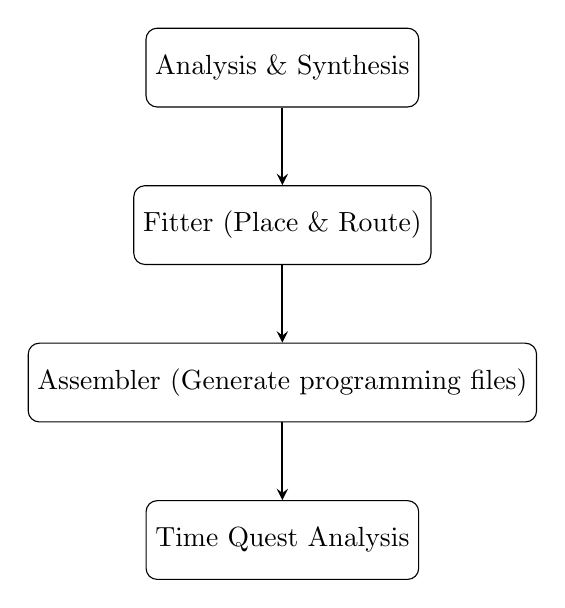
\begin{tikzpicture}[node distance=2cm]
	%defines
	\tikzstyle{systemDesign} = [rectangle, rounded corners, minimum width=3cm, minimum height=1cm,text centered, draw=black]
	\tikzstyle{ioIntegration} = [rectangle, rounded corners, minimum width=3cm, minimum height=1cm,text centered, draw=black]
	\tikzstyle{designDescription} = [rectangle, rounded corners, minimum width=3cm, minimum height=1cm,text centered, draw=black]
	\tikzstyle{synthesis} = [rectangle, rounded corners, minimum width=3cm, minimum height=1cm,text centered, draw=black]
	\tikzstyle{arrow} = [thick,->,>=stealth]
	%chart
	\node (systemDesign) [systemDesign] {Analysis \& Synthesis};
	\node (ioIntegration) [ioIntegration, below of=systemDesign] {Fitter (Place \& Route)};
	\node (designDescription) [designDescription, below of=ioIntegration] {Assembler (Generate programming files)};
	\node (synthesis) [synthesis, below of=designDescription] {Time Quest Analysis};
	\draw [arrow] (systemDesign) -- (ioIntegration);
	\draw [arrow] (ioIntegration) -- (designDescription);
	\draw [arrow] (designDescription) -- (synthesis);
\end{tikzpicture}
	\caption{FPGA design flow}\label{fig:fpgaCompileFlow}
\end{figure}
				\paragraph{SignalTap II Logic Analyzer:	}
When the configured FPGA doesn't work, SignalTap can help you. SignalTap is a logic analyser as shown in figure\ref{fig:signalTap}, where developers can review included signals. SignalTap needs two signals to be configured, the clock and a signal to trigger a ''hold''. Triggering conditions can be set on a signal by rising, falling of either edge. When the trigger condition occurs, all signals are plotted on a time span of a pre set number of clock cycles. Logic analyzers give a good look into systems with a high clock speed.
\begin{figure}
	\centering
	\includegraphics[scale=0.42]{images/SignalTapLogicAnalyzer.png}
	\caption{SignalTap II Logic Analyzer layout}
	\label{fig:signalTap}
\end{figure}
			\subsubsection{Operating system issues}
Quartus has some annoying issues. When using Quartus 16.1 installed on Red Hat 6.5, basic Verilog code and an OpenCL kernel can be compiled. Qsys, a tool to rapidly integrate IP of Altera in Quartus, gives synthesise errors during compilation. Those errors are really annoying, because an expensive commercial available program like Quartus should work in all times. So when there is an error, developers expect they created the error. Instead of Quartus creating error messages on his own. The solution was found by installing multiple versions of Quartus on both Linux and Windows, Quartus 16.1 installed on Windows 10 seemed to work perfectly with Qsys-tool, but the OpenCL kernel didn't compile anymore. Finally we used Quartus 16.1 installed on Windows 10 and Linux Red Hat 6.5 in order to successfully compile the system.
%%Bluetooth						%%%%%%%%%%%%%%%%%%%%%%%%%%%%%%%%
		\section{Bluetooth}
			\subsection{Master}
			\subsection{slave}
%%Web socket						%%%%%%%%%%%%%%%%%%%%%%%%%%%%%%%%
		\section{Web socket}

\bibliographystyle{IEEEtranS}
\bibliography{ThesisTUT}
\end{document} 